\documentclass[11pt,a4paper]{book}
\usepackage[utf8]{inputenc}
\usepackage[french]{babel}
\usepackage[left=2cm,right=2cm,top=2cm,bottom=2cm]{geometry}
\usepackage{fancyhdr}
\usepackage{appendix}
\usepackage{amsmath}
\usepackage{amsfonts}
\usepackage{amssymb}
\usepackage{stmaryrd}
\usepackage{mathrsfs}
\usepackage{graphicx}
\usepackage[ruled,vlined, french, algochapter]{algorithm2e}
\usepackage{ntheorem}
\usepackage[table,dvipsnames,svgnames]{xcolor}
\usepackage[framemethod=tikz]{mdframed}
\usetikzlibrary{shadows,shadings}
\usepackage{sectsty}
\usepackage{multicol}
\usepackage{hyperref}
\usepackage{listings}
\usepackage{float}
\usepackage[explicit]{titlesec}
\usepackage{colortbl}
\usepackage{enumitem}
\usepackage{tikz} %Tikz !
\usepackage{multirow}
\usepackage{ulem}
\usepackage{hhline}
\usetikzlibrary{automata, positioning, arrows}
\usetikzlibrary{shapes,shapes.geometric}
\usepackage{cancel}

\usepackage{xcolor}
\definecolor{mGreen}{rgb}{0,0.6,0}
\definecolor{mGray}{rgb}{0.5,0.5,0.5}
\definecolor{mPurple}{rgb}{0.58,0,0.82}
\definecolor{backgroundColour}{rgb}{0.95,0.95,0.92}

\tikzset{elliptic state/.style={draw,ellipse}}

% En-tête et pied de page
\newcommand{\mask}[1]{}

\pagestyle{fancy}
\renewcommand\headrulewidth{1pt}
\fancyhead[L]{Leçons d'Informatique}
\fancyhead[R]{Préparation à l'Agrégation d'Informatique 2022}
\fancyfoot[R]{\tiny $\copyright$ 2024 Martinez 2022 M. Marin}

\setcounter{tocdepth}{1} 



%Design des théorèmes
\usepackage{framed}


\newmdtheoremenv[
outerlinewidth=1pt,
innerlinewidth=0pt,
roundcorner=2pt,
linecolor=black,
shadow=true,
tikzsetting={shading=axis,top color=gray!10},
innertopmargin=1\baselineskip,
skipabove={\dimexpr0.5\baselineskip+\topskip\relax},
needspace=3\baselineskip ,
frametitlefont={\sffamily\bfseries},
]{theorem}%
{\color{BrickRed}Théorème}[chapter]

\newmdtheoremenv[
outerlinewidth=1pt,
innerlinewidth=0pt,
roundcorner=2pt,
linecolor=black,
shadow=true,
tikzsetting={shading=axis,top color=gray!10},
innertopmargin=1\baselineskip,
skipabove={\dimexpr0.5\baselineskip+\topskip\relax},
needspace=3\baselineskip ,
frametitlefont={\sffamily\bfseries},
]{proposition}%
{\color{IndianRed}Proposition}[chapter]

\newmdtheoremenv[
outerlinewidth=1pt,
innerlinewidth=0pt,
roundcorner=2pt,
linecolor=black,
shadow=true,
tikzsetting={shading=axis,top color=gray!10},
innertopmargin=1\baselineskip,
skipabove={\dimexpr0.5\baselineskip+\topskip\relax},
needspace=3\baselineskip ,
frametitlefont={\sffamily\bfseries},
]{lemma}%
{\color{IndianRed}Lemme}[chapter]

\newmdtheoremenv[
outerlinewidth=1pt,
innerlinewidth=0pt,
roundcorner=2pt,
linecolor=black,
shadow=true,
tikzsetting={shading=axis,top color=gray!10},
innertopmargin=1\baselineskip,
skipabove={\dimexpr0.5\baselineskip+\topskip\relax},
needspace=3\baselineskip ,
frametitlefont={\sffamily\bfseries},
]{corollary}%
{\color{IndianRed}Corollaire}[chapter]


\newmdtheoremenv[
outerlinewidth=1pt,
innerlinewidth=0pt,
roundcorner=2pt,
linecolor=black,
shadow=true,
tikzsetting={shading=axis,top color=gray!10},
innertopmargin=1\baselineskip,
skipabove={\dimexpr0.5\baselineskip+\topskip\relax},
needspace=3\baselineskip ,
frametitlefont={\sffamily\bfseries},
]{definition}%
{\color{ProcessBlue}Définition}[chapter]


\newmdtheoremenv[
outerlinewidth=1pt,
innerlinewidth=0pt,
roundcorner=2pt,
linecolor=black,
shadow=true,
tikzsetting={shading=axis,top color=gray!10},
innertopmargin=1\baselineskip,
skipabove={\dimexpr0.5\baselineskip+\topskip\relax},
needspace=3\baselineskip ,
frametitlefont={\sffamily\bfseries},
]{principe}%
{\color{DarkGreen}Principe}[chapter]


\makeatletter
\def\newframedGtheorem#1{%
\theoremprework{
\renewcommand*\FrameCommand{%
  {\color{DimGrey}\vrule width 3pt \hspace{2.5pt}}}
  \framed}%
\theorempostwork{\endframed}%
\newtheorem@i{#1}%
}
\makeatother
%%%


%Définition des différents environnements
\newframedGtheorem{rem}{\color{DimGrey}Remarque}[chapter]
\newframedGtheorem{com}{\color{Blue}Commentaire}[chapter]
\newtheorem{example}{\textbf Exemple}[chapter]
\newtheorem{exercise}{\color{orange}\textbf Exercice}[chapter]
\newtheorem{idee}{\textbf Idée}[chapter]
\newtheorem{temps}{\color{gray} Temps}[chapter]


\newtheorem{notion}{\textbf Notion}[chapter]
\newtheorem{algo}{\textbf Algorithme}[chapter]


\newtheorem{impl}{\textbf Implémentation}[chapter]
\newtheorem{syntaxe}{\textbf Syntaxe}[chapter]
\newtheorem{appl}{\textbf Application}[chapter]
\newtheorem{idea}{\textbf Idée}[chapter]

\newenvironment{proof}[1][\unskip]{\noindent \textit{Démonstration #1. }}{\hfill $\square$ \\}


%Gestion de la hierarchie
\setcounter{secnumdepth}{3}

\renewcommand{\familydefault}{\sfdefault}
\renewcommand{\thesection}{\arabic{section}}
\renewcommand{\thesubsection}{\Roman{subsection}}
\renewcommand{\thesubsubsection}{\Alph{subsubsection}}


\makeatletter
\renewcommand{\@chapapp}{Leçon}
\makeatother


%En-tête des leçons 
% utilisation : \debut{Auteurs}{niveau}{pré-requis}{références}
\newcommand\debut[4]{
\noindent \textbf{Auteur\textperiodcentered e\textperiodcentered s:} #1  \\
\noindent\textbf{Niveau :} #2 \\
\noindent\textbf{Pré-requis :} #3 \\
\noindent\textbf{Références :} #4 \\
}

%En-tête des développements 
% utilisation : \debut{Auteurs}{références}
\newcommand\dev[2]{
\noindent \textbf{Auteur\textperiodcentered e\textperiodcentered s:} #1  \\
\noindent\textbf{Références :} #2 \\
}

%Commande personnalisées
\newcommand{\N}{\ensuremath{\mathbb{N}}}
\newcommand{\overarrow}[1]{\smash{\overset{#1}{\longrightarrow}}}
\newcommand*\circled[1]{\tikz[baseline=(char.base)]{
		\node[shape=circle,draw,inner sep=2pt] (char) {#1};}}

%Pour le listing de code
\lstset{
frame = single, 
framexleftmargin=1pt,
literate=
{à}{{\`a}}1
{é}{{\'e}}1
{è}{{\`e}}1
{ô}{{\^o}}1}

\lstset{escapeinside={<@}{@>}}

\definecolor{lightpink}{HTML}{f7d1d5}
%Éviter le saut de page après un chapitre
\renewcommand{\cleardoublepage}{\newpage}
\newcommand\countme{\refstepcounter{\thechapter}\thechapter}

\lstdefinestyle{CStyle}{
	backgroundcolor=\color{backgroundColour},   
	commentstyle=\color{mGreen},
	keywordstyle=\color{magenta},
	numberstyle=\tiny\color{mGray},
	stringstyle=\color{mPurple},
	basicstyle=\footnotesize,
	breakatwhitespace=false,         
	breaklines=true,                 
	captionpos=b,                    
	keepspaces=true,                 
	numbers=left,                    
	numbersep=5pt,                  
	showspaces=false,                
	showstringspaces=false,
	showtabs=false,                  
	tabsize=2,
	language=C
}
%Copyright




\begin{document}

\begin{titlepage}
    \newgeometry{left=5cm,right=1cm,bottom=1cm}
    \noindent
\begin{flushright}
\vspace*{-3cm}

\includegraphics[scale=0.5]{Headers/logo-ens.png}
 
 \vspace{2cm}
\end{flushright}
    {\LARGE \textsf{École Normale Supérieure de Lyon} }
    \par
    \noindent
    \makebox[0pt][l]{\rule{1.3\textwidth}{1pt}}
    \par\medskip
    {\noindent \huge\textbf{\textsf{Leçons d'Informatique}}}
    \par\medskip
    {\noindent\huge\textbf{\textsf{Agrégation 2022} }}


    \par\vspace*{1cm}
    {\noindent\huge\textsf{Marin Malory, Sorci Émile, Rousseau Guillaume, Bertrand Jules} }
    

\vfill%

\end{titlepage}

\restoregeometry
\nopagecolor

\tableofcontents

\chapter*{Préface}
%\input{Préface/préface.tex}

\part{Leçons}

%\chapter{Exemples de méthodes et outils pour la correction des programmes.} \label{L1}
%\dev{Emile Martinez}{}{}{}

La conjecture de Syracuse est un problème ouvert de Mathématiques : \\
La suite $u$ définie par : $\left\{ \begin{array}{l}
	u_0 = a \in \N^*\\
	u_{n+1} = \left\{\begin{array}{ll}
		\dfrac{u_n}{2} & \text{si } u_n \text{ est pair}\\
		3u_n+1 & \text{sinon}
	\end{array}\right.
\end{array}\right.$ finie-t-elle toujours par le cycle $1,2,4$ ? (toujours = pour tout $a\in \N^*$)\\

Cela revient à savoir si l'algorithme \\
\begin{algorithm}[H]
	\caption{Syracuse(a)}
	$u \gets a$\\
	\Tq{$u$ est une nouvelle valeur}{
		\eSi{$u$ est pair}
		{
			$u\gets \dfrac{u}{2}$
		}{
			$u \gets 3u+1$
		}
	}
	\Retour{$u$}
\end{algorithm}
renvoie toujours 1, 2 ou 4.

\subsection{Terminaison}
Une première question est de savoir si \texttt{Syracuse} finit (ne boucle pas à l'infini) sur toute entrée.

\begin{definition}
	Prouver la terminaison d'un algorithme revient à prouver que sur toute entrée il termine
\end{definition}

\begin{rem}
	On se limite parfois aux entrées valides (pour Syracuse, $a \in \N^*$ par exemple)
\end{rem}

\begin{example}
	\enspace \\ \\
	\begin{minipage}{0.4\linewidth}
		\begin{lstlisting}
Tant que a > 0:
    a = a - 1
		\end{lstlisting}
	\end{minipage} \quad \begin{minipage}{0.5\linewidth}
		Termine sur tout entrée si on n'autorise pas $a$ à valoir $+\infty$, sinon ne termine pas sur toute entreé.
	\end{minipage}
\end{example}

\begin{definition}
	Un \textbf{variant} est une fonction des variables, à valeurs dans $\N$ qui décroit strcitement :
	\begin{itemize}
		\item à chaque passage dans la boucles pour les algorithmes itératifs
		\item à chaque appel récursif pour les algorithmes récursifs.
	\end{itemize}
\end{definition}

\begin{example} \enspace \\ \\ \label{1-2}
	\begin{minipage}{0.5 \linewidth}
		\begin{algorithm}[H]
			\caption{pgcd($a$,$b$)}
			\Tq{$\min(a,b) > 0$}{
				\eSi{$a<b$}
				{
					$b\gets b-a$
				}
				{
					$a\gets a - b$
				}
			}
			\Retour{$\max(a,b)$}
		\end{algorithm}
	\end{minipage} \quad \begin{minipage}{0.4 \linewidth}
		La fonction \texttt{pgcd(a,b)} qui calcule le pgcd de $a$ et $b$ pour $a, b \in \N$ admet comme variant $a+b$ (qui est en effet toujours positif, et décroit à chaque fois)
	\end{minipage}
\end{example}

\begin{proposition}
	\label{1-1}
	Si une boucle a un variant de voucle, alors elle s'éxecute un nombre fini de fois. De même pour un algorithme récursif.
\end{proposition}

\begin{example}
	pgcd($a$,$b$) termine pout tout $(a,b)\in \left(\N^*\right)^2$
\end{example}

\begin{rem}
	Si un algorithme termine sur toute entrée, il existe toujours un variant, mais il peut être difficile à trouver (ou à prouver)
\end{rem}

\begin{com}
	Il suffit de prendre comme variant le nombre d'étapes de calcul restantes en focntion de l'état de la mémoire
\end{com}

\begin{example} \enspace \\
	\begin{minipage}{0.4\linewidth}
		On définit $ack(n,m)$ pour $n,m\in \N$ par \\ $\left\{\begin{array}{l}
			ack(0,m) = m+1\\
			ack(n, 0) = ack(n-1, 1)\\
			ack(n,m) = ack(n-1, ack(n, m-1))
		\end{array}\right.$
	\end{minipage}\quad
	\begin{minipage}{0.55\linewidth}
		\begin{algorithm}[H]
			\caption{ack($n$,$m$)}
			\eSi{$n=0$}{
				\Retour{$m+1$}
			}{
				\eSi{$m = 0$}
				{
					\Retour{ack($n-1$, $m$)}
				}
				{
					\Retour{ack($n-1$, ack($n$, $m-1$))}
				}}
		\end{algorithm}
	\end{minipage} \\Il n'est pas immédiat que $ack$ termine.
\end{example}

\begin{definition}
	On dit qu'un ordre est un \textbf{ordre bien fondé} si toute suite décroissante est stationnaire
\end{definition}

\begin{example}
	$\N$ avec l'ordre naturel est bien fondé 
\end{example}

\begin{proposition}
	Les ordres produit et lexicographiques d'ordre bien fondés sont bien fondés
\end{proposition}

\begin{example}
	Un ordre total sur un ensemble fini est bien fondé, donc l'ordre alphabétique est bien fondé (c'est un ordre lexicographique)
\end{example}

\begin{definition}
	On étend alors la définition du variant aux fonctions à valeurs dans un bon ordre.
\end{definition}

\begin{proposition}
	La propriété \ref{1-1} reste valide avec notre définition étendue du variant
\end{proposition}

\begin{example}
	Pour ack, $(n,m)$ est un variant dans $\N^2$ avec l'ordre lexicographique, donc ack termine
\end{example}

\subsection{Correction partielle}

Une autre question pour \texttt{Syracuse} est de savoir si on peut tomber sur un autre cycle que 1,2,4 et donc renvoyer autre chose que 1,2 ou 4.

\begin{definition}
	On appelle \textbf{spécification} d'un algorithme deux propriétés $P_1$ sur les entrées (pré-condition) et $P_2$ sur les sorties (post-condition)
\end{definition}

\begin{example}
	Pour Syracuse, $P_1 : «a\in \N»$ et $P_2 : «\text{Syracuse}(a) \in \{1,2,4\}»$
\end{example}

\begin{definition}
	On dit qu'un algorithme est \textbf{partiellement correct} si pour toute entrée vérifiant la pré-condition, si l'algorithme termine, la sortie vérifie la post-condition.
\end{definition}

\begin{example}
	L'algorithme de l'exemple \ref{1-2} est partiellement correct si la pré-condition est «$a\in \N, b \in \N$» et la post-condition «\texttt{pgcd(a,b)} renvoie le PGCD de a et de b» \label{1-3}
\end{example}

\subsubsection{Correction partielle des algorithmes impératifs}

Pour prouver la correction partielle des langages impératifs, on utilise un invariant de boucle.

\begin{definition}
	Un invariant de boucle est une propriété qui est vrai avant la boucle, et si elle est vraie quand on commence un tour de boucle, alors elle l'est quand on le finit.
\end{definition}

\begin{proposition}
	Si un invariant de boucle est valide, alors il est vrai après la boucle, et la condition d'arrêt de la boucle est fausse.
\end{proposition}

\begin{example}
	Pour pgcd, «$PGCD(a,b) = PGCD(a_0, b_0)$» où $a_0$ et $b_0$ sont les valeurs initiales de \texttt{a} et \texttt{b}, est un invariant valide.
	
	A la fin de l'exécution, on a donc $\min(a,b) = 0$ et $PGCD(a,b) = PGCD(a_0, b_0) = PGCD(\min(a,b), \max(a,b)) = PGCD(0, \max(a,b)) = \max(a,b)$. D'où l'assertion de l'exemple \ref{1-3}
\end{example}

\subsubsection{Correction partielle des algorithmes récursifs}


\begin{principe}
	Pour prouver la correction partielle d'un algorithme récursif, on vérifie que si \begin{itemize}[label=$\bullet$]
		\item la pré-condition est vérifiée
	\end{itemize}, alors
	\begin{itemize}[label=$\bullet$] 
		\item on ne fait que des appels récursifs où les arguments vérifient la pré-condition
		\item Si la post-condition des appels récursifs est vérifiée, alors celle de notre appel est vérifiée
	\end{itemize}
	\label{1-5}
\end{principe}

\begin{theorem}
	Si le principe \ref{1-5} est respecté, alors l'algorithme est partiellement correct.
\end{theorem}

\begin{example}
	\label{1-7}
	exp($a$,$n$) pour $a,n\in \N$ renvoie $a^n$.\\\\
	\begin{minipage}{0.5\linewidth}
		\begin{algorithm}[H]
			\caption{exp($a$, $n$)}
			\eSi{$n=0$}{
				\Retour{$1$}
			}{
				$x =$exp($a$, $n$)\\
				\eSi{$n$ est pair}
				{
					\Retour{$x*x$}
				}
				{
					\Retour{$x*x*a$}
				}
			}
			\end{algorithm}
	\end{minipage} \quad \begin{minipage}{0.4\linewidth}
		Précondition : «\texttt a est un flottant et \texttt n un entier».\\
		Postcondition : $\texttt{exp(a,n)} = a^n$.\\
		Alors, la pré-condition est valide à chaque appel, et comme $a^n = a^{\lceil n \rceil} * a^{\lfloor n \rfloor}$, le principe \ref{1-5} est respecté dans tous les cas donc l'algorithme est partiellement correct.
	\end{minipage}
\end{example}

\subsection{Correction}

La conjecture de Syracuse dit donc que notre fonction Syracuse termine, et quand elle termine est correcte (i.e. partiellement correcte).

\subsubsection{Cas général}

\begin{definition}
	Quand un programme termine sur toute entrée valide et est partiellement correct, on dit qu'il est correct, ou encore totalement correct.
\end{definition}

\begin{example}\enspace\\
	\begin{algorithm}[H]
		\caption{fusion($L_1$, $L_2$)}
		$res \gets []$\\
		$i,j \gets 0$\\
		\Tq{
			$i < |L_1|$	et $j < |L_2|$
		}{
			\eSi{$L_1[i] < L_2[j]$}{
				$res$.ajouter($L_1[i]$) \\
				$i \gets i + 1$
			}{
				$res$.ajouter($L_2[j]$) \\
				$j \gets j + 1$
			}
		}
		Ajouter le reste de $L_1$ et de $L_2$ à $res$\\
		\Retour{$res$}
	\end{algorithm}

	\begin{algorithm}[H]
		\caption{tri\_fusion($L$)}
		$n \gets |L|$\\
		\Si{$n\leq 1$}{
			\Retour{$L$}
		}
		$L_1, L_2 \gets$ partionner($L$)\\
		\Retour{fusion( tri\_fusion($L_1$), tri\_fusion($L_2$) )}
	\end{algorithm}
\end{example}

\textbf{Developpement \ref{D?}} Correction totale de tri\_fusion.\\

Néanmoins, ce n'est pas toujours facile. La conjecture de Syracuse est toujours un problème ouvert. Et c'est parfois même pire.

\begin{theorem}
	La correction partielle et la terminaison sont indécidables. \label{1-6}
\end{theorem}

\textbf{Developpement \ref{D?}} Preuve du théorème \ref{1-6}

\subsubsection{Cas des algorithmes récursifs}

Dans le cas des algorithmes récurifs, on fait régulièrement la correction totale directement.

\begin{proposition}
	SI $(E, \preceq)$ est un ordre bien fondé, alors toutes parties non vides à un élément minimal (plus grand que personne)
\end{proposition}

\begin{theorem}
	\label{1-4}
	Soit $(A, \preceq)$ un ensemble muni d'un ordre bien fondé et $\mathcal P$ une propriété sur $A$, alors $\forall x \in A, \, (\forall y \in A, \, y \preceq A \enspace \Rightarrow \enspace \mathcal P(y) \Rightarrow \mathcal P(x)) \enspace \Rightarrow \enspace \forall x ,\, \mathcal P(x)$
\end{theorem}

\begin{rem}
	Cela étend le principe de réccurence forte sur $\N$
\end{rem}

L'ordre bien fondé nous donne alors le variant et la propriété l'invariant. On montre alors la terminsaison et la correction partielle en même temps.

\begin{example}
	Dans l'exemple \ref{1-6}, la propriété $\mathcal P(n)$ : «exp($a$,$n$)$ = a^n$» vérifie les bypothèses du théorème \ref{1-4}. Donc, $\forall n, \texttt{exp(a,n)} = a^n$, et ce pour tout $a\in \N$
\end{example}

\begin{com}
	Ici on suppose que exp($a$,$n$)$ = a^n$ veut dire que exp termine et renvoie $a^n$
\end{com}

\subsection{Outils}

\begin{itemize}[label=$\star$]
	\item Typer : Le fait d'utiliser un typage fort comme en OCamL permet d'éviter beaucoup d'erreurs bêtes
	\item Programmer défensivement en utilisant la bibliothèque assert.h permet de vérifier qu'à un moment donné du code, les hypothèses (ou les invariants) sont satisfaits (et pas seulement une erreur aléatoires parmi 1000 lignes)
	\item Faire des test tout au long de la programmation, en utilisant au maximum la modularité, pour détecter le plus tôt possible les erreurs.
	\item Utiliser des logiciels comme GDB ou valgrind pour détecter les fuites mémoires, ou l'inspecter au cours du programme.
	\item Commentez ! C'est primordial pour déclarer la spécification des fonctions et rendre le code compréhensible, donc déboguable.
\end{itemize}
%
%\chapter{Paradigmes de programmation : impératif, fonctionnel, objet. Exemples et applications.} \label{L2}
%\dev{Emile Martinez}{}{}{}

Programmer, c'est mettre en relation un cahier des charges et des instructions compréhensibles par la machine.
\begin{definition}
	Un \textbf{paradigme de programmation} définit la façon d'approcher la programmation informatique.
\end{definition}

Suivant le contexte il en existe plusieurs que nous verrons ici.


\subsection{La programmation impérative}

C'est la plus classique.

\begin{definition}
	La \textbf{programmation impérative} consiste à donner une suite d'instructions, chacune ayant pour seul effet de modifier l'état du programme (la mémoire, la valeur des variables, l'endroit où on en est etc...).
\end{definition}

\begin{rem}
	Ainsi, dans la programmation impérative, il n'existe pas de valeurs de retour. Si on en veut une, il faut écrire la valeur que l'on veut dans la mémoire.
\end{rem}

\begin{rem}
	Informellement, programmer impérativement, c'est utiliser des variables, des affectations, des tableaux, des boucles for et while, etc...
\end{rem}

\begin{example}
	La majorité du code en python est impératif\\\\
	\begin{minipage}{0.2\linewidth}
		\begin{lstlisting}
x = 1
y = x + 3
while (x != y):
    print(y)
    y -= 1
		\end{lstlisting}
	\end{minipage} \quad \begin{minipage}{0.75 \linewidth}
		Ce programme écrit 1 dans la case mémoire de x, puis y accède pour écrire 4 dans celle de y, puis écrit la valeur de y dans l'espace mémoire dédié à l'affichage, etc...
	\end{minipage}
\end{example}

\begin{rem}
	Impératif est pris ici dans son sens courant (en informatique). Une autre définition d'impératif est qu'on dit exactement ce que la machine doit faire (ex : l'assembleur), ce qui s'opose alors au déclaratif (comme SQL). Mais cette notion est à degré (dans tous langage il y a une marge plus ou moins grande pour la machine) et n'est pas nécessairement celle à laquelle on pense quand on pense à de la programmation impérative (même si les deux sont très liées).
\end{rem}

\subsection{Programmation fonctionnelle}

\begin{definition}
	La \textbf{programmation fonctionnelle} consiste à composer le programme de fonctions
	(au sens mathématiques), et de récupérer la valeur de retour.\\
	Les changements d'état ne peuvent pas être représentés par des évaluations de fonctions, donc la programmation fonctionnelle ne les admet pas. On dit que les structures de données fonctionnelles sont immuables.
\end{definition}

\begin{example}
		\lstinline|let max (x,y) = if x > y then x else y| \\ (fonction de type \lstinline|int*int -> int|) \label{2-1}
\end{example}

Informellement, programmer en fonctionnel, c'est considérer les fonctions comme des objets comme les autres, et n'avoir que des structures de données immuables.

\begin{rem}
	Un argument d'une fonction ou la valeur de retour d'une fonction peut être une fonction. C'est ce que l'on appelle la  programmation d'ordre supérieure.
\end{rem}

\begin{definition}
	La \textbf{curryfication} est la transformation d'une fonction à plusieurs arguments en une fonction à un argument qui retourne une fonction sur le reste des arguments
\end{definition}

\begin{example}
	On peut transformer la fonction \lstinline|max| de l'exemple \ref{2-1} en la fonction \lstinline|let max x y = if x > y yhen x else y de type int -> int -> int| \label{2-2}
\end{example}

\begin{example}
	Si, sur l'exemple \ref{2-2}, on veut que max puisse comparer des éléments sur lesquels on ne connait pas l'ordre, on peut en faire une fonction d'ordre supérieur en lui fournissant une fonction de comparaison : \\
	\lstinline|let max compar x y = if compar x y then x else y| de type \lstinline|('a -> 'a -> bool) -> 'a -> 'a -> 'a|\\
	On a alors \begin{itemize}[label =]
		\item \lstinline|max (fun x y -> x > y)| qui calcule le max 
		\item \lstinline|max (fun x y -> x > y) 3| qui est une fonction de type \lstinline|int -> int| renvoyant le maxmimum de son argument et 3
		\item \lstinline|max (fun x y -> x < y)| qui calcule le min
	\end{itemize}
\end{example}

\begin{rem}
	La puissance du fonctionnel vient de la récursivité
\end{rem}

\subsection{Programmation orientée objet}

\subsubsection{Obtenir de la modularité}

\begin{definition}
	Une \textbf{classe} est un ensemble de types de données appelés \textbf{attributs} et de \textbf{fonction} appelées méthodes. \newline
	Un \textbf{objet} est un représentant d'une classe. C'est un espace en mémoire contenant les valeurs des différentes attribut, les méthodes étant communes à tous les objets.
\end{definition}

\begin{example} \label{2-3}\enspace \\ \\
	\begin{minipage}{0.60 \linewidth}
		\begin{lstlisting}
class Noeud:
    def __init__(self, x):
        self.valeur = x
    def afficher(self):
        print(self.valeur)
    def est_egal(self, autre):
        return self.valeur == autre.valeur
a = Noeud(5)
a.afficher()
		\end{lstlisting}
	\end{minipage}\quad \begin{minipage}{0.35\linewidth}
		Ici Noeud est une classe, valeur un attribut de la classe Noeud, afficher et est\_egale des méthodes de la classe Noeud et a un objet (représentant) de la classe Noeud
	\end{minipage}
\end{example}

\begin{definition}
	La \textbf{programmation orienté objet} consiste à utiliser des classes et des objets de ces classes quand on programme.
\end{definition}

\begin{rem}
	Une utilisation massive des classes et de permettre de la modularité : on peut avoir une interface entre un type abstrait et son utilisation, rendant l'utilisation et la structure implémentant le type indépendant.
\end{rem}

\begin{example}
	En python, le package numpy propose les objets numpy.array que l’on crée via la commande
	a = numpy.array([...]). Un tel objet possède des attributs comme sa taille (a.size) mais aussi des
	méthodes tq a.sort()). Cette classe implémente des tableaux de taille fixe et de nombreuses méthodes dessus. On peut les utiliser en ne comprenant rien à comment elles fonctionnent, seulement ce qu'elles font, mais on peut aussi les réimplenter sans rien changer à l'utilisation de ces tableaux par des millions de personnes.
\end{example}

\subsubsection{Pour résoudre un problème}

Une autre utilité de la programmation orienté objet, et de représenter un problème avec ses différents objets que l'on fera intéragir entre eux.

\begin{example}
	Sur l'exemple \ref{2-3}, on peut rajouter la classe \lstinline|Arbre| contenant des noeuds.
	\begin{lstlisting}
class Arbre:
    def __init__(self, n, liste_arbre):
        self.noeud = n
        self.fils = liste_arbre
    def afficher(self):
        n.afficher()
        for x in self.fils:
        x.afficher()
	\end{lstlisting}
\end{example}

\subsection{Dans la vraie vie ?}

\subsubsection{Le multiparadigme}

	Dans la vraie vie, la plupart des langages de programmation implémente plusieurs paradigmes. En effet, python, comme C ou Ocaml, permettent de faire des boucles while, de faire des tableaux, de faire des structures et des fonctions récurisves, et même les fonctions d'ordre supérieur dans une certaine mesure.\\
	
	On appelle cela le multiparadigme. Néanmoins, certains langages sont plus adapatés à certains paradigmes, eux-mêmes plus adaptés à certaines contraintes.\\
	
	Des langages comme C, C++, Fortran, python, Java sont des langages impératifs, quand Haskell, ML, OcamL sont fonctionnels. De plus, python, C++ sont orientés objets.

\subsubsection{Comparaison des paradigmes}
	\begin{itemize}[label=$\star$]
		\item Pour des structures récursives comme des arbres (ou des graphes peu denses), le paradigme fonctionnel est approprié
		\item Le paradigme fonctionnel offre également élégance et lisibilité au code, avec moins d'instructions «superflues»
		\item Le caractère intrinséquement modulaire et sans effet de vord le rend aussi plus facile à tester et sécuriser : C'est en OcamL (en Coq) qu'est implémenté CompCert, un compilateur C vérifié.
		\item La programmation impérative est beaucoup plus proche de la machine et rend donc la compilation plus simple, et le développement intelligent potentiellement plus efficace.
		\item Il est aussi très performant pour des structures de données séquentilles et des accès «aléatoires» à des données. Par exemple représenter une matrice, en faire des multiplications, etc... paraît beaucoup plus simple en C qu'en OcamL.
		\begin{exercise}
			Implémenter un tas min en C et en OCamL
		\end{exercise}
		\item L'orienté objet est quant à lui de plus haut niveau et repose souvent sur d'autres paradigmes plus bas niveau.
		\item Il est souvent utilisé pour représenter des situtations complexes grâce à sa modularité
		\begin{exercise}
			Implémenter les classes représentant un personnage de jeu vidéo, ses objets, ses compétences, etc...
		\end{exercise}
	\end{itemize}

\subsubsection{Et SQL ?}

	Il existe néanmoins bien d'autres paradigmes, comme par exemple le paradigme logique, où seul le résultat est présenté par le code, et non la manière de l'obtenir. C'est par exemple le cas du SQL pour les bases de données, où l'exécution n'est pas dicté par la requête, seul son sens l'est, laissant le SGBD se charger du déroulement.
%
%\chapter{Tests de programme et inspection de code.}
%\label{L3}
%\dev{Emile Martinez, Malory Marin}{}{}{}

\section{Introduction}

\subsection{Qu'est-ce qu'un test}

Tester est un anglicisme pour le mot français essayer (ou éprouver). Me soumettant à la folie anglomane ambiante je garderai ce mot, soucieux de ma cohérence avec le monde extérieur.

\begin{definition}
	\textbf{Tester} un programme consiste à essayer d'y trouver des erreurs
\end{definition}

\begin{rem}
	On ne cherche pas ici à prouver directement que le programme est correct, mais à prouver qu'on n'arrive pas à se rendre compte qu'il est incorrect.
\end{rem}

\subsection{Données de tests}

\begin{definition}
	\textbf{Une donnée de test} est un couple (valeur d'entrée, valeur de sortie), où à l'évidence, le deuxième élément représente la valeur de sortie quand la fonction est appelée sur le premier élément.
\end{definition}

\begin{definition}
	\textbf{Un jeu de données de test} (ou jeu de tests) est alors un ensemble de tels couples, permettant de vérifier la validité du programme sur certaines entrées.
\end{definition}

\begin{rem}
	Certaines sorties (attendues) peuvent être des erreurs.
\end{rem}

\begin{example}
	Un jeu de tests pour une fonction calculant le pgcd peut être \\$\left\{ \big((1,2), 1\big), \big((-3, 6), 3\big), \big((0, 0), 0\big), \big((2, 2.45), \text{Erreur de type}\big) \right\}$
\end{example}

\subsection{Types de tests}

Il existe deux types de tests : 
\begin{itemize}
	\item Les tests en boites noires : On ne connait pas le code de la fonction, on peut simplement l'appeler. 
	\item Les tests en boites blanches : On connait le code et on génère un jeu de test en fonction. 
\end{itemize}

\section{Tests en boîtes noires}

\subsection{Caractéristiques}

Pour un test en boîtes noires, comme on ne connait pas le code, il faut tester beaucoup de données. Idéalement, toutes, mais cela se trouve souvent impossible.

\begin{example}
	On peut tester toutes les valeurs d'une fonction qui implémente une fonction booléenne mais pas celles de notre fonction calculant le pgcd de deux nombres
\end{example}

Viennent alors deux problèmes : Générer suffisament de données d'entrées et effectuer le test suiffisament rapidement.

\subsection{Générer des données d'entrée}

Dans de nombreux cas, ne pouvant pas essayer toutes les données d'entrées, on va devoir faire des choix.

\begin{idee}
	La première approche consisterait à générer des valeurs aléatoires dans un domaine, et espérer en prendre suffisamment pour que cela fonctionne.
\end{idee}

\begin{principe}
	Une approche plus maline, à partitionner le domaine, puis à appliquer l'approche naïve sur chaque domaine.
\end{principe}

\begin{example}
	Pour le calcul de pgcd($a$,$b$), on peut parititionner le domaine d'entrées en comparant $a$, $b$, et $0$, (avec donc 6 domaines : $a <= 0 <= b$, $0 <= a <= b$, $0 <= b <= a$, $a <= b <= 0$, $b <= a <= 0$, $b <= 0 <= a$)
\end{example}

\begin{rem}
	On se contente souvent de prendre un seul test par classe.
\end{rem}

\begin{rem}
	Le choix du partitionnement est arbitraire et doit donc être fait suivant la manière d'approcher le problème
\end{rem}


Une fois cela fait, il est très commun que les erreurs puissent venir des cas limites. 

\begin{principe}
	On essaye alors de se placer au limites des domaines, et de vérifier spécifiquement ces cas là.
\end{principe}

\begin{example}
	Pour l'exemple précédent, on testerai les cas d'égalité : $0 <= a = b$, $a = 0 = b$, $a  = 0 <= b$ etc... (en effet par exemple, le cas 0, 0 est différent des autres, la valeur pouvant être $+\infty$ ou $0$ suivant les définitions).
\end{example}

\subsection{Utiliser les caleurs de sorties efficacement}

Néanmoins, maintenant que l'on a les valeurs d'entrées, il faut pour avoir notre jeu de tests avoir également les valeurs de sorties.

\begin{example}
	si l'on veut générer la sortie du pgcd sur des entrées que l'on a pris au hasard, il faut connaitre déjà le pgcd. Quel intérêt d'avoir notre fonction alors si on a déjà une fonction qui le fait
\end{example}

\noindent On a alors plusieurs méthodes : \begin{enumerate}
	\item Générer un jeu de tests à la main
	\item Utiliser un programme moins performant mais que l'on sait correct.
	\begin{example}
		Si on calcule le pgcd par soustraction successives, on peut tester en calculant le pgcd en testant tous les nombres inférieurs à $a$ et a garder le plus grand qui divise $a$ et $b$.
	\end{example}
	\item Ne pas calculer la réponse mais simplement vérifier que la réponse fourni est correcte.
	\begin{example}
		Si on a un programme qui nous donne la décomposition en facteurs premiers d'un nombre, il nous suffit de tester la primalité de chaque sortie et de vérifier que leur produit fait l'entrée.
	\end{example}
\end{enumerate}

\begin{example}
	Si on a un algorithme performant effectuant le produit de matrice, on peut : \begin{enumerate}
		\item Créer à la main quelque petite matrice et faire leur produit pour vérifier que tout fonctionne
		\item Comparer avec l'algorithme naif du calcul de produit de matrice
		\item Vérifier de manière probabiliste que le résultat est bien le bon.\\
		\textbf{Developpement \ref{D?}} Vérification probabiliste du produit de matrice.
	\end{enumerate}
\end{example}

\section{Tests en boite blanche}

\subsection{Graphe de flot de contrôle}

Pour un test en boîte blanches, on connaît le code, et on va vouloir générer des données d'entrées en fonction de ce code là.\\

Pour cela, on extrait du code le graphe de flot de contrôle.

\begin{definition}
	Le graphe de flot de contrôle est un graphe où chaque boîte contient des lignes de codes, les boites sont reliés si on peut exécuter l'une puis l'autre.
\end{definition}

\begin{example}
	\label{3-1}
	On prend l'exemple du pgcd pour $a, b \in \N^*$\\
	
	\noindent \begin{minipage}{0.5\linewidth}
		\begin{algorithm}[H]
			\Tq{$a \neq b$}{
				\eSi{$a < b$}{
					$b \gets b - a$
				}{
					$a \gets a - b$
				}
			}
			\Retour{$a$}
		\end{algorithm}
	\end{minipage}\begin{minipage}{0.5\linewidth}
		\begin{tikzpicture}[->, node distance=2cm]
			\node[elliptic state, scale = 1] (q0) {Début};
			\node[elliptic state, scale = 1, below right of = q0] (q1) {$a \neq b$};
			\node[elliptic state, scale = 1, above right of = q1] (q2) {Fin};
			\node[elliptic state, scale = 1, below left = 0.8cm and 1.5cm of q1] (q3) {$b \gets b - a$};
			\node[elliptic state, below right = 0.8cm and 1.5cm of q1] (q4) {$a \gets a - b$};
			\node[elliptic state, below right = 0.8cm and 1.5cm of q3] (q5) {$a < b$};
			
			\draw (q0) edge[] node{} (q1);
			\draw (q1) edge[left] node{Oui} (q2);
			\draw (q1) edge[left] node{Non} (q5);
			\draw (q3) edge[] node{} (q1);
			\draw (q4) edge[] node{} (q1);
			\draw (q5) edge[left] node{Oui} (q3);
			\draw (q5) edge[right] node{Non} (q4);
		\end{tikzpicture}
	\end{minipage}
\end{example}

\subsection{Utilisation du graphe}

On essaye alors de générer un jeu de données qui parcourt une bonne partie du graphe.

Par exemple, un jeu couvrant : \begin{itemize}
	\item Tous les nœuds (On veut un jeu de tests tel que tous les tests pris ensemble, chaque nœud du graphe est parcouru au moins une fois).
	\item Tous les arcs
	\item Tous les chemins
\end{itemize}

\begin{com}
	Si on veut aller plus loin, on peut aussi rajouter toutes les conditions décisions, toutes les p utilisations, etc... On peut alors rajouter un exercice proposant de montrer la hiérarchie entre ces tests.
\end{com}

\begin{example}
	Sur l'exemple \label{3-1}, $\left\{ \big( (1,1), 1\big), \big((1,3), 3)\big)\right\} $ ne couvre pas tous les nœuds quand $\left\{ \big((1,3), 3), \big( (3, 1), 3 \big) \right\}$ couvre tous les nœuds et tous les arcs mais pas tous les chemins.
\end{example}

\begin{rem}
	Quand il y a une boucle, tous les chemins peut-être un critère infini. On peut alors se limiter aux chemins d'une certaine taille.
\end{rem}

\begin{rem}
	Parfois les critères sont insatisfiables.
\end{rem}

\begin{rem}
	Aucun de ces critères ne garantissent la validité d'un algorithme. Elles permettent simplement de vérifier que notre jeu de tests n'est pas trop lacunaire.
\end{rem}

\noindent \textbf{Developpement \ref{D?}} Intérets et insuffisances de ces critères

\subsection{Test exhaustif de condition}

\begin{idee}
	Une autre approche consiste à avoir un jeu qui satisfait ou invalide toutes les conditions de toutes les manières possibles.
\end{idee}

\begin{example}
	On voit l'utilité sur l'exemple suivant :\\
	\begin{minipage}{0.5\linewidth}
		\begin{lstlisting}[style=CStyle]
int max(int a, int b){
	if(a > b || a == 500){
        return a;
    else
        return b;
}
\end{lstlisting}
	\end{minipage}
	\begin{minipage}{0.5\linewidth}
		Pour détecter le problème (que max ne calcule pas le $\max$), il faut des tests où on mets à vrai le premier if à cause de $a == 500$, donc des tests où $a$ vaut $500$.
	\end{minipage}
\end{example}

\section{Pratiques pour éviter d'avoir à déboguer}


Dans la pratique, de bonne pratique de code sont très efficace pour éviter de passer trop de temps à debugguer son code.

\begin{itemize}[label=$\star$]
	\item Compiler avec -Wall (activant tous les warnings, donnant beaucoup de bugs stupides)

	\item Respecter la ponctuation et éventuellement utiliser un linter (de manière à rendre lisible le code par d'autres personnes)

	\item Faire de la programmation défensive en utilisant assert par exemple
\end{itemize}


%
%\chapter{Principe d'induction}
%\label{L4}
%\dev{Emile Martinez}{}{}{}

\section{Principe}
\subsection{Definition}

\begin{definition}
	$(\mathcal B, (f_i))$ est une signature sur $X$ si : \begin{itemize}	
	\item $\mathcal B \subset X$ (appelé cas de base)
	
	\item $f_i : X^{\alpha(i)} \to X$ appelé constructeurs, d'arité $\alpha(f_i)$ avec $f_i$ injectif et $\Im(f_i) \cap \Im(f_j) = \empty$ et $\Im(f_i) \cap \mathcal B = \empty$ pour tout $i \neq j$
	\end{itemize}
\end{definition}

\begin{com}
	L'intérêt de cette définition est d'être rigoureux. Néanmoins le programme demande de se contenter de présenter des choses proches de ce que l'on rencontrera, or là c'est plus ou moins la version formelle de ce qui se passe en OcamL. Donc meme si ce cadre théorique n'est pas explicitement au programme, sa présence là est justifiée par sa proximité avec OcamL
\end{com}

\begin{rem}
	On se contente souvent de dire que les constructeurs existent, sans donner leur définition. (de même pour les cas de bases, et pour X) \label{4-3}
\end{rem}

\begin{example}
	\label{4-1}
	On prend une constante $Z$ et un constructeur d'arité 1 $Succ$
\end{example}

\begin{example}
	\label{4-2}
	On peut prendre les constructeurs $\oplus$, $\ominus$ $\otimes$ et $\otimes$ avec $\alpha(\oplus) = 2$, $\alpha(\ominus) = 1$ et $\alpha(\otimes) = 2$ et comme cas de bases $\N$. 
\end{example}

\begin{definition}
	\label{4-4}
	Un ensemble inductif est définit par une signature $(\mathcal B, (f_i))$: \begin{enumerate}
		\item Le plus petit ensemble contenant $\mathcal B$ et stable par tous les $f_i$ (définition par le haut)
		
		ou de manière équivalente
		
		\item $\bigcup T_i$ où $T_0 = \mathcal B$ et $T_{n+1} = T_{n} \cup \bigcup\limits_{i} f_i( T_{n} ^ {\alpha(f_i)})$ (définition par le bas)
	\end{enumerate}
\end{definition}

\begin{example}
	L'ensemble inductif définit par l'exemple \ref{4-1} peut être une définition des entiers naturels \label{4-6}
\end{example}

\begin{example}
	Exemple : L'ensemble inductif $\mathcal A_{simp}$ définit par l'exemple $\ref{4-2}$ est l'ensemble des expressions arithmétiques simplifiées.
\end{example}

\begin{rem}
	$\oplus(1, 1) \neq \otimes(1, 2) \neq \otimes(2, 1)$. On s'intéresse à l'expression et non au résultat.
\end{rem}

\noindent \textbf{Développement \ref{D?}} Validité de la construction d'un ensemble inductif (remarque \ref{4-3} et définition \ref{4-4})

\subsection{Induction structurelle}
On prendra maintenant $(\mathcal B, (f_i)_{i \in I})$ une signature.

\begin{proposition}
	\label{4-5}
	Soit $E$ un ensemble inductif construit par $(\mathcal B, (f_i))$\\
	
	Alors la donné de fonction $g_i$ (avec $\alpha(g_i) = \alpha(f_i)$ et $\Im(g_i) \subset Dom(g_j)$ ) et de $f(b)$ pour $b \in \mathcal B$ définit une unique fonction $f$ sur $E$ ayant la propriété:
	$$\forall i \in I, \forall x_1, \, \dots , \, x_{\alpha(i)} \in X, \, f\left(f_i(x_1, \, \dots, \, x_{\alpha(i)})\right) =  g_i\left(f(x_1), \dots, \, f(x_{\alpha(i)})\right)$$
\end{proposition}

\begin{com}
	Cette propriété est fondamentale, et justifie en partie (parce que la il ne faut pas un matching complet mais directement les constructeurs) la bonne définition des fonctions OcamL. D'où d'ailleurs les références à cette propriété dans la suite.
\end{com}


\begin{example}
	Sur $\mathcal A_{Simp}$, on peut définir $eval : \mathcal A_{Simp} \to \N$ par \begin{itemize}
		\item $eval(a) = a$ pour $a \in \N$
		\item $eval(\oplus(a, b)) = eval(a) + eval(b)$
		\item $eval(\otimes(a, b)) = eval(a) \times  eval(b)$
		\item $eval(\ominus(a)) = - eval(a)$
	\end{itemize}
\end{example}

\begin{theorem}[Induction structurelle]~
	Soit $E$ l'ensemble inductif définit par $(\mathcal B, (f_i)_{i\in I})$, et $\mathcal P$ une propriété définie pour tout $x\in E$.\\
	
	Alors $\left\{ \begin{array}{cl}
		(i) & \forall b \in \mathcal B, \mathcal P(b)\\
		(ii) & \forall i \in I, \, \forall x_1, \, \dots, x_{\alpha(i)}, \, \left( \forall j, \, \mathcal P(x_j)\right) \implies \mathcal P \big( f_i(x_1, \, \dots, \, x_{\alpha(i)})\big)
	\end{array} \right.$	
\end{theorem}

\begin{rem}
	La récurrence est un cas particulier dans le cas de la définition des entiers par l'exemple \ref{4-6}
\end{rem}

\begin{example}
	On montre par induction structurelle que $eval(e)$ pour $e \in \mathcal A_{simp}$ est multiple du pgcd des constantes apparaissant dans $e$
\end{example}

\begin{definition}
	Un ordre bien fondé est un ordre où toute partie non vide admet un élément minimal (plus grand que personne)
\end{definition}

\begin{proposition}
	L'ordre produit et l'ordre lexicographique d'ordres bien fondés sont bien fondés
\end{proposition}

\begin{example}
	$\N$ avec l'ordre naturel est bien fondé, donc $\N^k$ avec l'ordre produit ou lexicographique aussi.
\end{example}

\begin{theorem}
	Soit $(A, \preceq)$ un ensemble muni d'un ordre bien fondé et $\mathcal P$ une propriété sur $A$, alors $\forall x \in A, \, (\forall y \in A, \, y \preceq A \enspace \Rightarrow \enspace \mathcal P(y) \Rightarrow \mathcal P(x)) \enspace \Rightarrow \enspace \forall x ,\, \mathcal P(x)$
\end{theorem}

\begin{rem}
	Cela étend le principe de réccurence forte.
\end{rem}

\begin{definition}
	Soit $E$ l'ensemble inductif défini par $(\mathcal B, (f_i)_{i \in I})$
	
	On définit l'ordre structurel $\leq_s$ sur $E$ comme la clôture transitive réflexive de $x_j \leq_s f_i(x_1, \, \dots, \, x_{\alpha(i)})$
\end{definition}

\begin{proposition}
	$\leq_s$ est une relation d'ordre bien fondé
\end{proposition}

\begin{corollary}
	On peut alors réécrire l'induction structurelle comme une induction sur l'ordre structurelle
\end{corollary}

\begin{com}
	Si on manque de place, on peut mettre les ordres bien fondés en prérequis (mais alors écrire la formule dans le corollaire)
\end{com}

\subsection{En OCaml}

\begin{com}
	On essaye de faire au maximum le lien entre les définitions formelles et OcamL
\end{com}

\begin{syntaxe}
	En OcamL on peut créer un type représentant un ensemble inductif avec cette syntaxe :
	\begin{lstlisting}
type  t = Casdebase1 | Casedebase2 | ... 
        | Constructeur1 of type11 *type12 * .... 
        | Constructeur2 of type21 * tpye22 * ...
	\end{lstlisting}
	
	Où : \begin{itemize}
		\item \texttt{Casdebase} peut soit être un type déjà défini d'OcamL, soit une constante (nom commençant par une majuscule)
		\item \texttt{Constructeur} est une étiquette commencée par une majuscule 
		\item \texttt{typei} est est un type OCamL (pouvant contenir \texttt t)
	\end{itemize}
\end{syntaxe}

\begin{example}
	Pour définir les entiers de l'exemple \ref{4-6}, on peut écrire \begin{lstlisting}
type entier = Zero | Succ of entier
	\end{lstlisting}
\end{example}

\begin{syntaxe}
	Pour gérer les types, on peut utiliser le filtrage comme pour les listes.
\end{syntaxe}

\begin{example}
	Pour l'addition sur notre type entier, on peut écrire :
	\begin{lstlisting}
let rec ajouter x y = match y with
  | Zero -> x
  | Succ(z) -> ajouter (Succ(x)) z
	\end{lstlisting}
\end{example}

\begin{example}
	La validité de cette définition vient de la propriété \ref{4-5}
\end{example}

\section{Structures de données inductives}

\subsection{Les listes chaînées}


En OcamL on peut définir des listes d'entier simplement chaînés par \begin{lstlisting}
type liste = V | Cons of int * liste
\end{lstlisting}

Ainsi, une liste c'est soit une liste vide, soit un entier et le reste de la liste.

\begin{rem}
	Ici \texttt V est le cas de base, et \texttt{Cons} le constructeur. $Cons$ est défini sur $\N \times \{\text{ensemble des listes}\}$ et non $\{\text{ensemble des listes}\}^2$. Cela est un raccourci d'OCamL, où en réalité on définit un constructeur pour chaque premier argument, et donc on construit non pas $Cons(x, l)$ mais $Cons_x(l)$.
\end{rem}

\begin{rem}
	Cela correspond au type \texttt{int list} d'OCamL ;-)
\end{rem}

\begin{exercise}
	Définir inductivement la taille d'une liste chaînée
\end{exercise}

\subsection{Les arbres binaires}

\begin{exercise}
	Définir inductivement la taille d'une liste chaînée.
\end{exercise}

\begin{definition}[Arbre binaires]
	Soit $A$ un ensemble. On définit de manière inductive les arbres binaires sur $A$ par : \begin{itemize}
		\item l'arbre vide $E$ (cas de base)
		\item si $e\in A$ et $g$ et $d$ sont des arbres binaires, alors $Noeud(e,g,d)$ est un arbre binaire.
	\end{itemize}
\end{definition}

\begin{impl}
	Ce qui en OCamL nous donne \texttt{type 'a arbre = E | Noeud of 'a * 'a arbre * 'a arbre}
\end{impl}

\begin{example}
	La hauteur d'un arbre binaire se calcule alors inductivement par \begin{lstlisting}
let rec hauteur arb = match arb with
  | E -> 0
  | Noeud(e, g, d) -> 1 + max (hauteur g) (hauteur d)
	\end{lstlisting}
\end{example}

\begin{exercise}
	Prouver par induction structurelle la terminaison de la fonction hauteur
\end{exercise}

\begin{exercise}
	Donner la définition inductive de la taille d'un arbre binaire (son nombre d'éléments)
\end{exercise}

\subsection{Les arbres généraux}

\begin{definition}
	Un arbre général est un noeud (la racine) et une liste d'arbre (ses fils)
\end{definition}

On voudrait alors définir le type \texttt{arbre} par (pour les arbres d'entier)
\begin{lstlisting}
type arbre = Noeud of int * arbre_liste
\end{lstlisting}
Il faut alors définir le type \texttt{arbre\_liste}, par
\begin{lstlisting}
type arbre_liste = Vide | Cons of arbre * arbre_liste
\end{lstlisting}

On remarque que chaque type a besoin de l'autre pour exister. On écrit alors
\begin{lstlisting}
type arbre = Noeud of int * arbre_liste
and type arbre_liste = Vide | Cons arbre*arbre_liste
\end{lstlisting}

\begin{rem}
	On passe souvent cela sous le tapis grâce au polymorphisme qui définit des manières de construire des types et non des types directement
\end{rem}

\begin{com}
	Dans la défense de plan, on peut parler ici des différentes définition des arbres (par coinduction, avec une infinité de constructeur (pour chaque $k \in \N^*$ d'arité $k$, pour les arbres à $k$ fils), par un constructeur $Ajout\_fils$ d'arité 2 où le premier argument est l'arbre sans son premier fils, et le dernier argument le premier fils (on en déduit les cas de bases))
\end{com}

\section{Ensembles inductifs}

\subsection{Formules propositionnelles}

\begin{definition}[formule propositionelle]~
	Soit $V$ un ensemble de variables et la signature \begin{itemize}
		\item $\mathcal B = \{ \top, \bot\} \cup V$
		\item le constructeur $\neg$ d'arité 1
		\item les constructeurs $\vee$, $\wedge$ et $\to$ d'arité 2 (en forme infixe)
	\end{itemize}
	Les formules propositionnelles forment l'ensemble inductif défini par cette signature
\end{definition}

\begin{exercise}
	Défini inductivement le nombre de variables présent dans la formule
\end{exercise}

\begin{definition}
	On appelle valuation (ou distribution de vérité) toute fonction $v : V \to \{0, 1\}$
\end{definition}

\begin{definition}[Evaluation d'une formule] Soit $v$ une valuation. La fonction d'évaluation d'une formule $[.]_v : F \to \{0,1\}$ se définit inductivement par \begin{itemize}[label=$\bullet$]
		\item $[\top]_v = 1$
		\item $[\bot]_v = 0$
		\item $[x]_v = v(x)$ pour $x \in V$
		\item $[\neg F]_v = 1 - [F]_v$
		\item $[f_1 \wedge f_2]_v = \min([f_1]_v, [f_2]_v)$
		\item $[f_1 \vee f_2]_v = \max([f_1]_v, [f_2]_v)$
		\item $[f_1 \to f_2]_v = \left\{ \begin{array}{ll}
			0 & \text{si } [f_1]_v = 0 \text{ et } [f_2]_v = 1\\
			1 & \text{sinon}
		\end{array} \right.$
\end{itemize}
\end{definition}

\begin{exercise}
	Définir l'équivalence entre formules et montrer par induction structurelle que, à équivalence près, on peut ne garder que les constructeurs $\neg$ et $\vee$
\end{exercise}

\subsection{Langages}

\begin{com}
	Ici comme exemple on aurait aussi pu prendre les langages réguliers, cela est plus pertinent comme construction, mais nécessite d'avoir déjà les définitions de bases sur les langages. Et de plus trouver des inductions parait non trivial
\end{com}

\begin{definition}
	Soit $\Sigma$ un ensemble (appelé alphabet) fini et non vides d'éléments (appelés lettres). On définit inductivement l'ensemble des mots sur $\Sigma$, $\Sigma^*$ par la signature : \begin{itemize}
		\item $\varepsilon$ (le mot vide) comme cas de base
		\item Si $a \in \Sigma$ et $w \in \Sigma^*$, $wa\in \Sigma^*$
	\end{itemize}
\end{definition}

\begin{rem}
	On aurait aussi pu prendre comme définition de $\Sigma^*$, $\bigcup\limits_{n \geq 0} \Sigma^n$
\end{rem}

\begin{definition}
	La concaténation de deux mots $w_1, w_2 \in \Sigma^*$ se définit inductivement comme : \begin{itemize}
		\item $concat(w_1, \varepsilon) = w_1$
		\item $concat(w_1, w_2.a) = concat(w_1, w_2).a$
	\end{itemize}
\end{definition}

\begin{exercise}
	Montrer par induction structurelle que $concat(w_1, concat(a, w_2)) = concat(w_1.a, w_2)$ 
\end{exercise}

\chapter{Implémentations et applications des piles, files et files de priorité}
\label{L5}
\dev{Emile Martinez}{}{}{}

\subsection{Les piles}

\textbf{Rappel :} Une pile est une structure de données avec les méthodes \texttt{vide}, \texttt{est\_vide}, \texttt{empiler}, \texttt{depiler}.

\subsubsection{Implémentation par listes}

Cette manière est immédiate et donc naturelle.

\begin{exercise}[Au tableau avec participation des élèves]
	A quoi correspondent les opérations de bases de la pile sur une liste (à l'oral et éventuellement avec le dessin d'une liste simplement chaînés pour montrer les modifications).
\end{exercise}

Les listes étant naturelles en OCaml, nous les implémenterons de cette manière en Ocaml. Néanmoins cette pile est immuable.

\subsubsection{Implémentation par tableaux}

La deuxième manière est en utilisant un tableau. \\

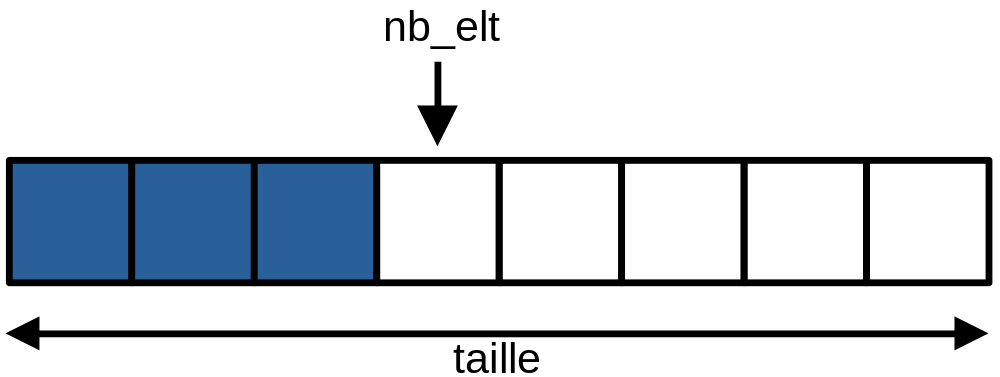
\includegraphics[scale=0.3]{lecon/05-piles_files/piles_tableau.png}
\\

\begin{principe}
	Pour cela, on utilise un indice \texttt{nb\_elt} qui nous indiquera à quelle case du tableau correspond le sommet de la pile, les cases précédentes du tableau contenant les autres éléments empilés.
\end{principe}

\begin{impl}
	On doit soit alors utiliser un tableau de taille fixe (et donc connaître à l'avance le nombre max d'éléments dans la pile)
\end{impl}

\makeatletter
\renewcommand{\@chapapp}{Développement}
\setcounter{chapter}{0}
\makeatother
\renewcommand\theHchapter{sec.\thechapter} %unique prefix

\part{Développements}
 

\end{document}
